\chapter{Mixed Reality for Human-Robot Collaboration}%
\label{chapter:on-site}
% \chapter{On-site Member's Application}% first title of section

\begin{introduction}
    This chapter presents the development of a comprehensive framework for implementing a Mixed Reality environment in Human-Robot Collaboration. 
    % By allowing both on-site and remote manipulation through a communication pipeline, this system enables real-time robot manipulation and monitoring. 
    The framework leverages advanced technologies such as Mixed-Reality, Digital Twins, and ROS, ensuring precise synchronization between physical and digital models. It discusses the tools, control methods, and User Interface enhancements designed to optimize both on-site and remote user experiences, aiming towards an intuitive, immersive collaboration.
\end{introduction}

\section{Framework}

Figure~\ref{fig:project_framework} illustrates the proposed framework of the \ac{MR}-based \ac{HRC} system. This framework seamlessly integrates two distinct environments—on-site and remote—through a robust communication pipeline designed to enable real-time, collaborative robot manipulation.

\begin{figure}[h]
    \centering
    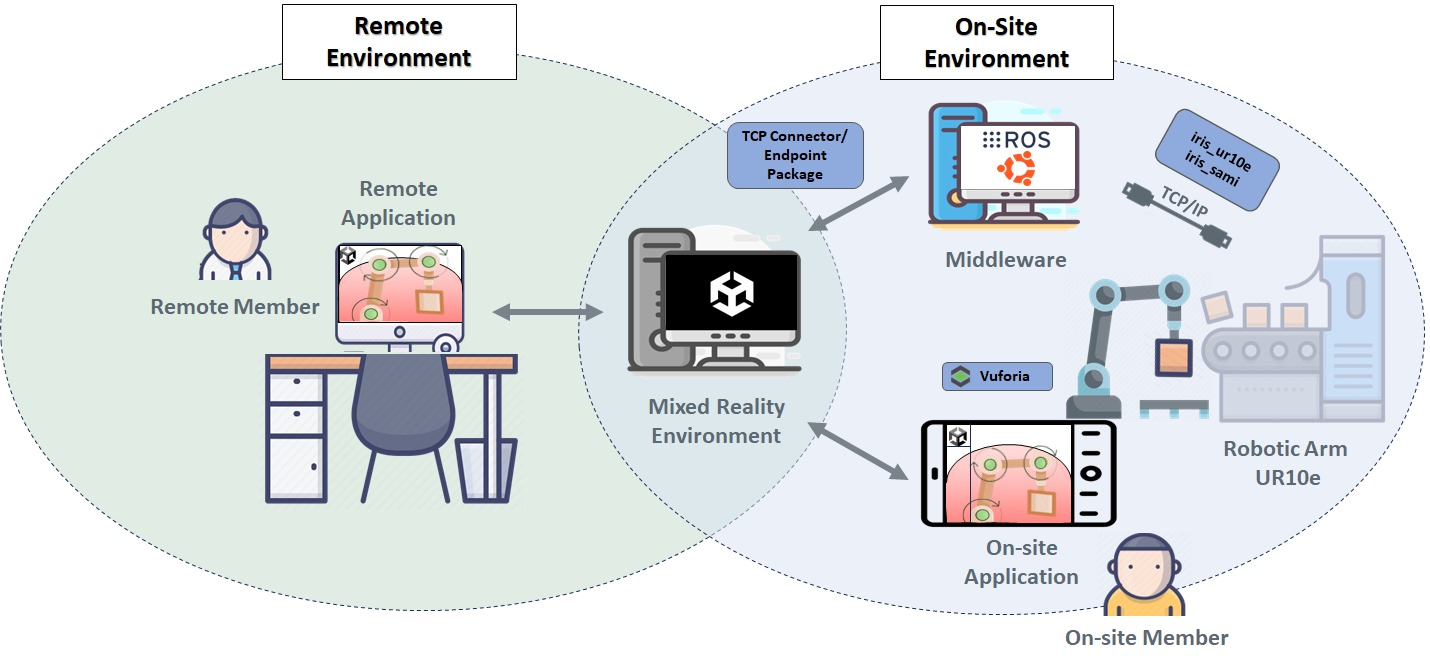
\includegraphics[width=\linewidth]{figs/framework-1.jpeg}
    \caption{Overview of the proposed \ac{MR}-based \ac{HRC} system framework integrating remote and on-site environments.}
    \label{fig:project_framework}
\end{figure}

First of all, regarding the \textbf{On-Site Environment}, the UR10e robotic arm operates as the central physical entity to be controlled and manipulated. The on-site user interacts with this robotic arm through a custom \ac{MR} application developed in Unity, chosen due to its robust \ac{MR} capabilities, which facilitate the creation of immersive, interactive environments, enabling intuitive real-time robot manipulation.

After implementing the robot digital model into the simulation environment, the next step was to align it with the physical robot. Pose registration between the physical robot and its digital counterpart is executed using Vuforia's capabilities. The system employs ArUco markers for precise pose estimation, ensuring that the digital representation of the UR10e is accurately aligned with its physical counterpart. The \ac{DT} of the robot, rendered in Unity, provides a visually synchronized, real-time mirror of the robot's movements and configurations, thus facilitating enhanced interaction.

The robot is connected via Ethernet to a laptop running Ubuntu 20.04 with \ac{ROS} Noetic, which serves as the middleware layer. This setup facilitates seamless data exchange between the Unity \ac{DT} and the physical robot. The \texttt{iris\_ur10e} and \texttt{iris\_sami} \ac{ROS} packages, developed by the IRIS Lab and available on GitHub\footnote{https://github.com/iris-ua}, provide a pre-established \ac{ROS} environment that supports critical functionalities such as trajectory planning and robotic manipulation and visualization through RViz.

To tailor these packages to the specific needs of this project, several enhancements were made. These modifications included the integration of bidirectional data flow between \ac{ROS} and Unity, enabling the Unity-based \ac{DT} to mirror the real-time movements of the physical robot. In particular, new \ac{ROS} nodes were created to subscribe to joint state data from the physical robot and publish these updates to Unity, ensuring precise synchronization between the physical and virtual environments. Additionally, new publishing mechanisms were implemented to send commands from Unity back to \ac{ROS}, allowing for full control of the robot through the \ac{MR} interface. These modifications were essential for realizing the bidirectional communication required for accurate \ac{DT} manipulation.

This communication between the \ac{ROS} middleware and Unity’s \ac{MR} environment is established using Unity’s \ac{ROS}-\ac{TCP}-Connector and \ac{ROS}-\ac{TCP}-Endpoint packages. These packages enable bidirectional communication over a \ac{TCP}/\ac{IP} protocol, ensuring real-time synchronization between the virtual and physical environments. This communication architecture is fundamental for maintaining the \ac{DT}'s fidelity, reflecting real-world changes in the Unity model and vice versa, as referred in the section \ref{sec:dt}.

Regarding the \textbf{Remote Environment}, a remote participant accesses the same Unity-\ac{MR} application. This allows the remote member to visualize and manipulate the robot in real time, from a separate location. The remote \ac{UI} provides real-time visualization of the robot’s state and its workspace, enabling remote collaboration. The synchronization between the remote and on-site environments is facilitated through Unity’s \ac{MR} capabilities, which, in conjunction with the \ac{ROS}-based control, enable the remote user to execute commands and receive real-time feedback.

The Middleware layer, acting as the system’s backbone, ensures the continuous synchronization of data between the physical robot and its \ac{DT}. It manages the real-time feedback loop, maintaining bidirectional data flow between the virtual robot in Unity and the physical robot in the on-site environment. This configuration guarantees that any actions performed by either the on-site or remote user are consistently reflected in both the physical and digital realms, preserving operational coherence and maximizing collaborative efficiency.

This framework provides an immersive and responsive \ac{MR} environment, bridging the gap between physical and digital spaces. The system enables real-time robot manipulation and monitoring from both on-site and remote locations, making it a versatile platform for collaborative tasks in advanced industrial applications. The seamless integration of \ac{MR}, \ac{DT}, and \ac{HRC} technologies significantly enhances user interaction, safety, and productivity, while offering an intuitive interface for remote and on-site collaboration.


% *TODO: see where to start explaining what was done regarding the control methods.
Three distinct control methods were developed within the application to facilitate manipulation, which will be explained further below.


\section{Mixed Reality Environment}

Regarding the Unity developed \ac{MR} environment, it started by implementing the proper UR10e digital model. This model was then aligned with the physical robot through Vuforia's pose registration capabilities, ensuring that the \ac{DT} would accurately mirror the robot movements and configurations.

The base robot manipulation provided by the \ac{URDF}-Importer package consisted on moving each joint individually by selecting the desired joint and then moving it with by using the keyboard directional arrows. This method was improved to three distinct control methods that enhance user experience and facilitate robot manipulation.

\section{Robot Manipulation}
In order to properly develop new ways of controlling the \ac{DT} version of the robot, it was necessary to understand the C\# script named \texttt{Controller.cs}, which contained all the necessary functions to control the robot's joints.


After further analysis, three methods were developed to control the robot's joints:
% \begin{itemize}
    % *TODO: add figures of: joint button selected and not selected (red and green)
    % *TODO: add figures of: joint direction selected and not selected (white and green)
    % * TODO: confirm if it is not possible to move the robot using other methods whenever the \ac{UI} interface is active. 
    % * TODO: add a figure of the toggle button activated and deactivated (green and gray) as well as the impact it has on the menu - showing it activated and deactivated (take a screenshot of the whole interface with the menu activated and deactivated)

    \subsection{UI Control}
    % \textbf{UI Control Method}:
    This method is designed to provide users with an intuitive, user-friendly interface for manipulating the \ac{DT} of the UR10e robot. 

    Figure \ref{f:ui-control} illustrates the \ac{UI} developed in Unity, highlighting its primary control panel on the left (1), which includes a detailed joint selection menu, directional arrows, and a reference image of the robot with joint labels (2 and 3). This panel is central to controlling the digital model of the robot, while other \ac{UI} features shown in the figure will be explained in subsequent sections.

    \begin{figure}[h]
        \centering
        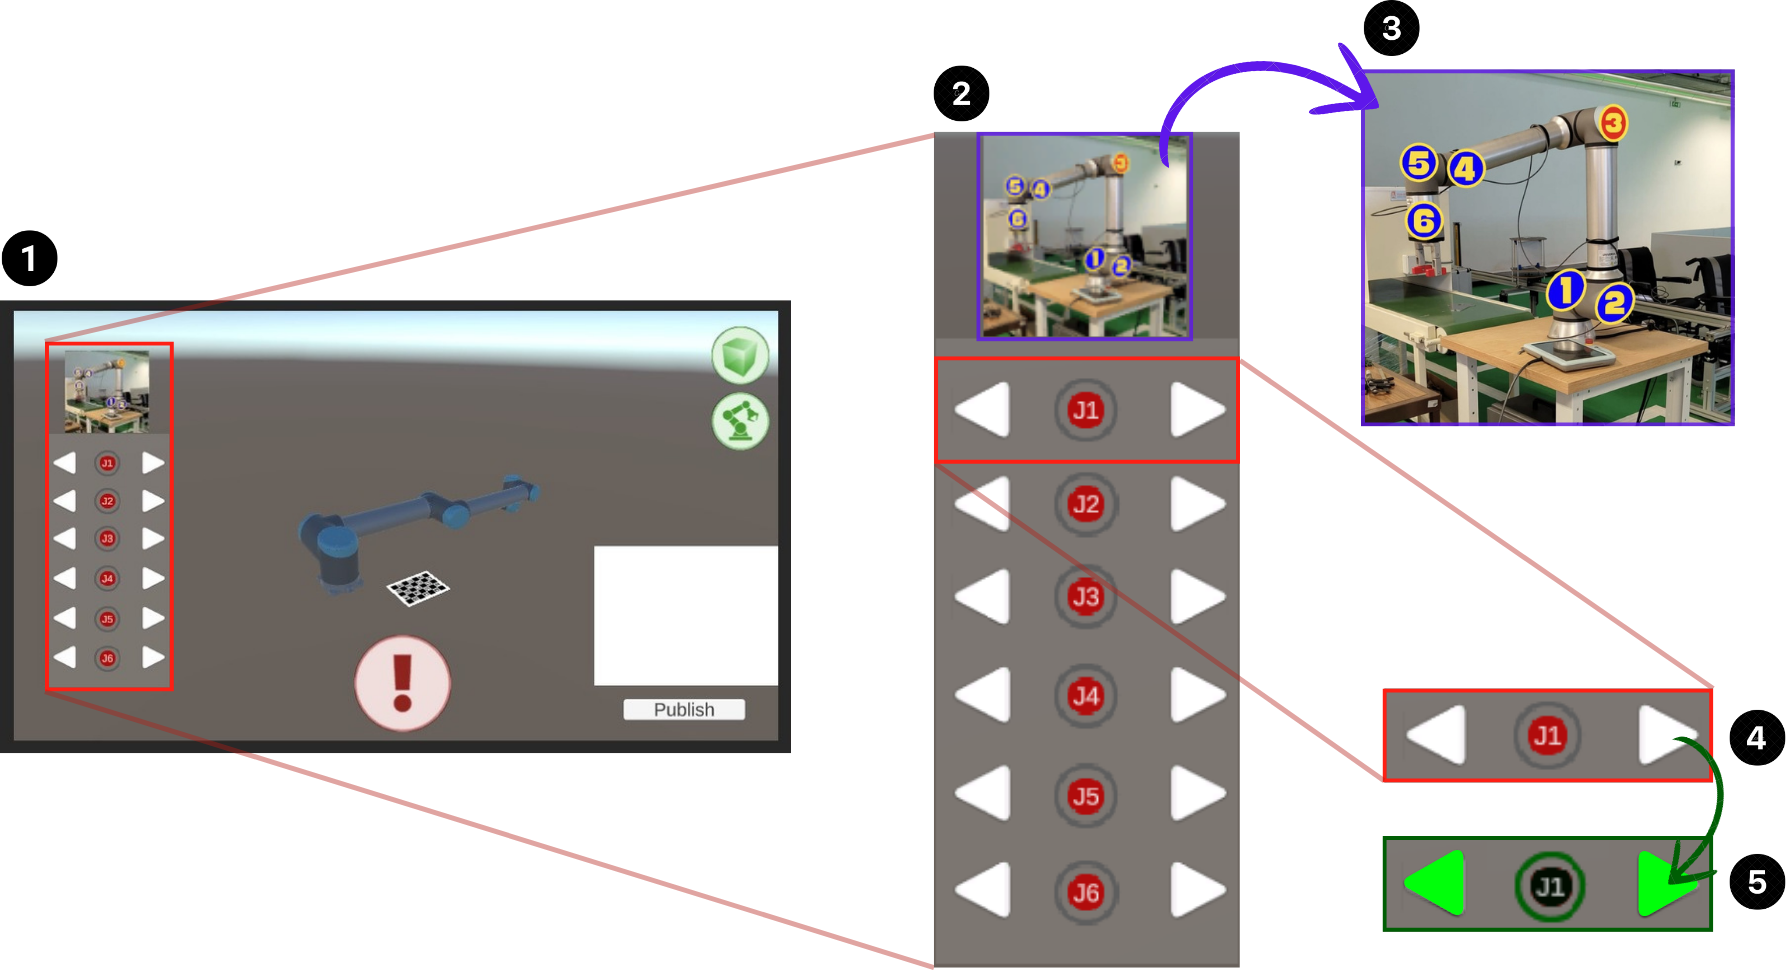
\includegraphics[width=\textwidth]{figs/interface-numerada-2.png}
        \caption{\ac{UI} panel (2) for the \ac{MR} Unity environment, enabling control of the digital model of the UR10e robot using the \ac{UI} Control method. Users can manipulate each joint individually, with active joints displayed in green to indicate selection (5). The reference image of the robot (3), labeled with joint numbers (J1 to J6), aids in joint identification from base to end-effector. Directional arrows for each joint (2,4,5) facilitate movement control in positive or negative directions, offering intuitive joint-level manipulation within the simulation.}
        \label{f:ui-control}
    \end{figure}

    \textbf{Interface Structure and Joint Manipulation}:
    \begin{itemize}
        \item \textbf{Joint Selection}: Each joint has a central button labeled with its identifier (e.g., J1, J2). To activate a joint, the user clicks the corresponding button, which changes color from red to green, signaling that the joint is selected for movement (4 and 5). This selection process helps avoid confusion and accidental manipulation of multiple joints.

        \item \textbf{Movement Control}: Once a joint is selected, the user can manipulate its position by clicking the directional arrows on either side of the central button. Pressing the right arrow rotates the joint in the positive direction, while the left arrow rotates it in the negative direction. This control mirrors the real-time responsiveness typically provided by keyboard arrows, ensuring an intuitive experience.

        \item \textbf{Continuous Movement}: The selected joint will continue moving in the chosen direction as long as its central control button and the directional arrow remain selected. To stop the movement, the user can simply deselect the joint by clicking the central button again, which reverts to its default color, or deactivate its rotation direction.
    \end{itemize}

    \textbf{Key Features and Operational Rules}:
    \begin{enumerate}
        \item \textbf{Single Joint Activation}: Only one joint can be active for rotation at any time. If multiple joints are selected (i.e., their buttons are green), the system prevents movement in any direction until only one joint is selected.

        % \item \textbf{Directional Exclusivity}: When a rotation direction is chosen (e.g., pressing the right arrow), the opposite direction is temporarily disabled, as shown in Figures 4 and 5. This feature prevents conflicting commands, reinforcing safe and logical control of the robot.
    \end{enumerate}

    \textbf{Additional Design Considerations}:
    \begin{itemize}
        \item \textbf{Visual Reference for Joint Positioning}: The overlay image at the top of the joint control panel serves as a quick-reference guide for users to confirm joint positions relative to the physical robot. This visual aid is useful in remote collaboration or complex tasks where clear identification of each joint’s location is essential.

        \item \textbf{UI Responsiveness and Feedback}: To ensure a smooth interaction, the interface provides visual feedback for each action (e.g., button color changes) and restricts movement based on user inputs, making the control process both transparent and manageable.
    \end{itemize}

    This structured approach to joint manipulation promotes safe, precise, and efficient interaction with the robot, supporting the usability goals of the \ac{MR} application. By minimizing the likelihood of accidental commands and providing continuous, clear visual feedback, the interface helps maintain control clarity and operational awareness throughout the interaction.
    % The design is especially advantageous in collaborative environments, where multiple participants may need to observe and understand the robot’s operations in real time.


    
    % \textbf{UI Control:} This method allowed the user to control the \ac{DT} version of the robot by moving each joint individually through an Unity \ac{UI}. Its purpose consisted on being user-friendly and an intuitive manner of controlling the robot. 
    
    % The final \ac{UI} that was used in the mixed reality application can be seen below. regarding the digital model control method, the main part of the \ac{UI} consists on the menu panel with the joints and the figure of the robot on top of it, as displayed in the 1 figure of the figure \ref{f:ui-control}. the remaining elements will be explained further below when introducing the advanced features that were implemented besides the robot manipulation. so the menu, represented in the left part of figure 1 can be seen in figure 2 as an up-close version. the top part of it shows a figure of the real ur10e robot with the joints relative position superimposed into the robot, allowing the user to identify which joint to control if he has some doubts. this robot's joint overlay is represented in the figure 3, where it is visible that the joint's count occurs as it is often refered in robotics, starting from the base and counting up until reaching the end-effector joint of the robot. below this, there is the UI menu that enables the digital model manipulation within the unity environment, where each row represents a joint and in order to properly interact with it, the central Joint x (x for each joint number) must be selected and afterwards, either by pressing the right or left arrow, the selected joint will rotate in the corresponding direction, either in the positive or negative direction. the figure 4 shows, again, an up-close view of the first joint properties as default, and in the figure below, number 5, the activation of this joint is shown. this is visible because both the central joint button that represent the joint selection is green, showcasing its selection, and both the right and left arrows are enabled, visible again by the change in its default color. However, it is not possible to rotate a robot's joint in both directions at the same time, so the developed interface only allows the user to manipulate one joint at a time, and in one direction. if the user activates the central button for more than one joint, and then tries to rotate one of the selected joints in any direction, the digital model will not perform this action. Is is necessary that only the desired joint must be activated with the central button as green.
    
    % we can see the menu interface on the left part represented by each joint ativation toggle button alognside with two directional arrows that enable the rotation movement either in the positive or negative direction of the selected joint. this control method was implemented in order to allow the robot to be manipulated through this menu interface. On the top part of this menu that allows the maniupulation of each joint individually, there is a image of the robot showing the relative number of each joint, just to clarify that the joint count starts from the bottom joint to the end-effector. this can also be seen in figure. upon selecting the specific joint, its button is activated and this can be seen by the change of its color.   
    
    
    % Apart from the joints' buttons, there is also a figure of the robot displayed in the top part of the panel, showing each joint's relative number, and thus allowing an easier identification of the joint to be controlled. This menu is displayed in the Figure~\ref{fig:}.
    
   
    % % \FloatBarrier

    % % Upon pressing a joint's respective button, its color changes from the default red to green, allowing the user to understand which joint is currently selected. Besides, the user can also choose between rotating the selected joint in either the positive or negative direction, which is also represented by a change in the default color of the corresponding directional arrow. These features are represented in Figure: 

    % In this control method, only a joint can be moved at a time, so whenever two joints are selected in the \ac{UI} menu, none of the remaining joints will be able to rotate.
    % The developed features of the \ac{UI} control method are described below:
    % \begin{itemize}
    %     \item \textbf{Joint Selection}: Users can activate a joint by clicking on it. Upon activation, the selected joint's central red circle turns green.
    %     \item \textbf{Movement Control}: By clicking on the selected joint's directional arrows within the interface, it moves in either a 
    %     positive or negative direction. This functionality mimics the real-time movement control similar to using keyboard arrow keys, ensuring 
    %     intuitive operation.
    %     \item \textbf{Continuous Movement}: The selected joint continues to move until we deactivate its respective button.
    %     \item \textbf{Single Joint Activation}: To ensure precise control, joint movement is only possible when one joint is selected at a time. 
    %     This prevents unintended actions and enhances the accuracy of adjustments.
    % \end{itemize}
    
   

    \subsection{Unity to Robot}
    % \textbf{Unity-ROS Control:} 
    Similarly to the previous described method, this one also enables the digital robot model to be controled from the \ac{MR} environment. However, when needed, it updates the newly defined digital robot position into the real on-site UR10e robot. In order to change the \ac{DT}, the user has to press the right/left arrow keyboard keys to select the following/previous joint as well as the up/down keys to rotate the selected joint in the positive/negative direction, respectively.
         
    After moving the digital model to the desired position, by pressing the "Publish" button within the \ac{UI}, as shown in Figure \ref{fig:publish_UI_button}, the robot's joints coordinates are published to the \ac{ROS} middleware, using the \ac{ROS}-\ac{TCP}-Connector/Endpoint packages.
    

    \begin{figure}[htpb]
        \centering
        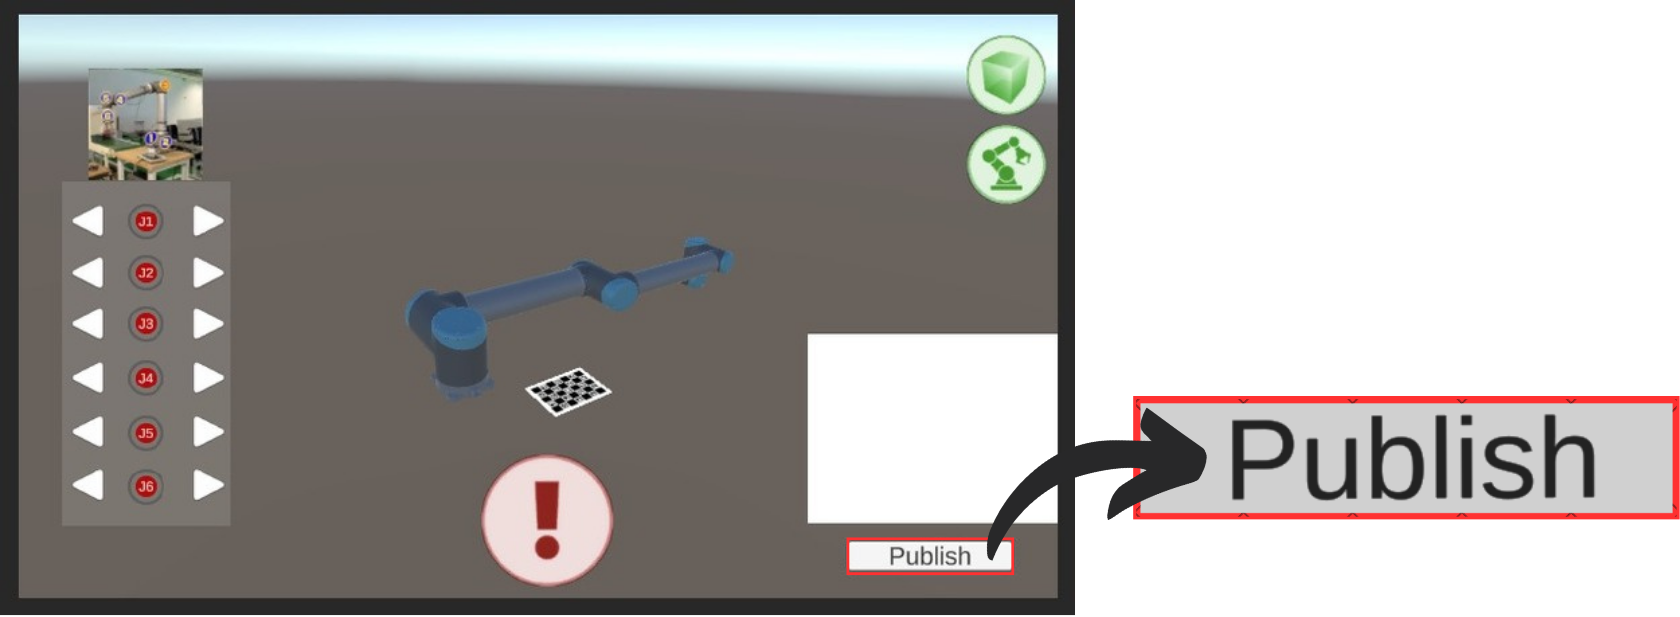
\includegraphics[width=\linewidth]{figs/publish-button.png}
        \caption{Publish button that sends Unity's \ac{DT} robot joint states into ROS the environment}
        \label{fig:publish_UI_button}
    \end{figure}

    To avoid conflicts with the \ac{ROS} node responsible for controlling the real robot's joints, which are being constantly published to the standard \texttt{joint\_states} topic, a separate \ac{ROS} topic \texttt{(unity\_joint\_states)} was created to handle the joint data coming from Unity. This ensures that data from Unity does not interfere with the real robot’s ongoing operations. When the "Publish" button is pressed, the Unity-defined joint states are sent to this new topic, and only when necessary are they relayed to the real robot for movement execution. Below, there is a pseudo-code snippet explaining how to update the \ac{DT} in Unity and send the new desired robot position to the \ac{ROS} middleware.

    \begin{algorithm}
        \caption{Unity Input for Joint Selection and Movement}\label{alg:unity_input}
        \begin{algorithmic}[1]
            \State \textbf{Step 1: User Input for Joint Selection and Movement in Unity}
            \While{Unity Simulation is running AND Unity-ROS Control is enabled}
                \If{RightArrowKeyPressed}
                    \State Select next joint
                \ElsIf{LeftArrowKeyPressed}
                    \State Select previous joint
                \EndIf
                \If{UpArrowKeyPressed}
                    \State Rotate selected joint in positive direction
                \ElsIf{DownArrowKeyPressed}
                    \State Rotate selected joint in negative direction
                \EndIf
                \If{PublishButtonPressed}
                    \State joint\_states = GetCurrentJointStates()
                    \State PublishToROSTopic('unity\_joint\_states', joint\_states)
                \EndIf
            \EndWhile
        \end{algorithmic}
    \end{algorithm}

    
    In order to handle this communication process, two new \ac{ROS} nodes were created, the \texttt{joint\_state\_listener} and the \texttt{move\_unity} nodes. The \texttt{unity\_joint\_subscriber.py} script was developed within the \texttt{iris\_ur10e} package, initializing the node that subscribes to the \texttt{unity\_joint\_states} topic, which receives a JointState message type. It then initializes the publisher for the \texttt{move\_joint\_unity} topic, converting this data into a Float64MultiArray format which will be further received by the second node. This second node called \texttt{move\_unity}, created within the \texttt{iris\_sami} package, subscribes to the \texttt{move\_joint\_unity} topic, listening to new joint position values, moving the robotic arm to this desired position. This real-time update can be visualized either on the simulation environment, through Rviz, or by utilizing the real UR10e robot. Another pseudo-code explanation regarding how both \ac{ROS} nodes work, is presented below.

    
    % The \texttt{unity\_joint\_subscriber.py} script was developed within the \texttt{iris\_ur10e} package.
    % By creating a new node, called \texttt{joint\_state\_listener}, it then subscribes to the \texttt{unity\_joint\_states} topic, expecting to receive a JointState message type.
    % Afterwards, it initializes a publisher for the \texttt{move\_joint\_unity} topic, that converts this data into a Float64MultiArray format that will be further received by the second node.
    
    % Regarding the second node, the \texttt{move\_unity.py} script was created in the . It initializes the \texttt{test\_arm\_movement} node that listens for joint position commands on the \texttt{/move\_joint\_unity} topic.
    % Upon receiving this data, it moves the robotic arm to the desired position.

    % Part 2: ROS Node for Receiving Unity Joint States

    \begin{algorithm}
        \caption{Combined ROS Node for Receiving Unity Joint States and Moving the Robot}\label{alg:combined_ros_node}
        \begin{algorithmic}[1]
            \State \textbf{Step 2 and 3: Combined ROS Node for Receiving Unity Joint States and Moving the Robot}
            
            % Initialize first node
            \State Initialize ROS Node: joint\_state\_listener
            \State Subscribe to Topic: 'unity\_joint\_states'
            
            \While{Receiving JointState message from Unity}
                \State float\_array\_data = ConvertToFloat64MultiArray(joint\_states)
                \State PublishToROSTopic('move\_joint\_unity', float\_array\_data)
            \EndWhile
            
            % Initialize second node dependent on the first node
            \State \textbf{Precondition:} The \texttt{joint\_state\_listener} node must be running and publishing to the \texttt{'move\_joint\_unity'} topic.
            \State Initialize ROS Node: test\_arm\_movement
            \State Subscribe to Topic: 'move\_joint\_unity'
            
            \While{Receiving Float64MultiArray message from \texttt{move\_joint\_unity}}
                \State MoveRobotArmTo(joint\_positions)
                \If{ConnectedToRealRobot}
                    \State MoveRealRobot()
                \Else
                    \State VisualizeInRviz()
                \EndIf
            \EndWhile
        \end{algorithmic}
    \end{algorithm}

    
        
    \subsection{Robot to Unity}
    * TODO: add here a figure of the Robot to Unity - real robot and superimposed dt in unity

    % \textbf{\ac{ROS}-Unity Control:}
    Opposite to the above described method which controlls the \ac{DT} and then updates the robot position, in this control method, the on-site user moves the robot and the remote counterpart visualizes this update instantly within the \ac{MR} environment.
    
    In order to properly achieve this communication and data transfer, the \texttt{JointStateSubscriber.cs} script was created in Unity. It subscribes to the \texttt{joint\_states} topic, and stores the information regarding the joint positions in a dictionary structure that is updated in real time into a specific \texttt{.json} file within the \ac{MR} environment. This file is constantly being read by the \texttt{Controller.cs} script whenever this control method is enabled, updating the \ac{DT} robot model accordingly.
    
    By maintaining this synchronization between the real robot and the virtual environment, the Unity scene accurately reflects the robot's live state, ensuring a consistent \ac{DT} representation through the bidirectional communication established between the \ac{MR} environment and the \ac{ROS} middleware. Below, there is another pseudo-code explaining how the \ac{ROS}-Unity control method works.


    \begin{algorithm}
        \caption{ROS-Unity Control via Joint States Subscription}\label{alg:ros_unity_control}
        \begin{algorithmic}[1]
            \State \textbf{Step 1: Subscribe to ROS \texttt{joint\_states} topic}
            \State Attach the Unity Script to the Digital Robot Model Asset: \texttt{JointStateSubscriber.cs}
            \State Upon Initialization, it subscribes to topic: \texttt{/joint\_states}
    
            \While{Receiving JointState message from \ac{ROS}}
                \State Extract joint names and positions from the message and store them in a dictionary data structure
                % \State Store them in a dictionary structure
                \State Save the dictionary data to the \texttt{jointStateSubscriber.json}
            \EndWhile
    
            \State \textbf{Step 2: Update Unity \ac{DT} Robot Model}
            \While{Simulation is Running}
                \State Read the \texttt{jointStateSubscriber.json}
                \State Update the Unity \ac{DT} robot model using the joint positions from the dictionary structure
            \EndWhile
    
            \State \textbf{Step 3: Synchronize Real Robot with \ac{DT} Robot}
            \State The Unity \ac{DT} robot model moves according to the real robot’s joint positions, ensuring a consistent bidirectional \ac{DT} representation.
        \end{algorithmic}
    \end{algorithm}
    
% \end{itemize}

 
\section{On-site Mixed-Reality Features}
\label{section:on-site-features}
% \input{chapters/on-site/on-site-features} commented this part because text is below - choose whether to use this or the text below
After having implemented the \ac{DT}-Robot bidirectional communication between the on-site and remote members, the next step consisted on developing features that could enhance both users' experience when interacting with the collaboration environment. These features were designed to improve user safety, facilitate robot manipulation, and provide an intuitive interface. The following sections detail these key features development and implementation.

% Regarding the on-site member's collaboration experience, as explained in the state of art review, by implementing different sensorial cues, such as visual and audio, it will enhance the user experience into a more intuitive and immersive way.
    
\subsection{Virtual Safety Zones}
\label{subsection:virtual-safety-zones} 
% \input{chapters/on-site/subsections/virtual-safety-zones} commented this part because text is below - choose whether to use this or the text below

As explained in section \ref{sec:hrc-in-industry}, introducing different sensorial cues enhances on-site users' experience into a more intuitive and immersive experience. Therefore, visualizing the working zone of the robot is a critical feature designed to enhance safety when interacting with the robot. In order to achieve this, two safety zones were developed, as shown in Figure \ref{fig:blinking-sign}. 
* TODO: re-do this figure with the most recent version of the UI and safety-zones


Addressing specific safety and user experience concerns: 

\begin{itemize}
\item \textbf{Outer Safety Zone:} Initially, only this safety zone was created. The purpose of creating it was to provide an 
early warning to users as they approach the hazardous area near the robot. This approach consisted on changing its color as a visual alert. 
However, this method proved ineffective because, once inside it, users could not perceive the color change, rendering the warning system inadequate.

\item \textbf{Inner Safety Zone:} To overcome this outer zone limitation, an additional Inner-Safety Zone was developed. This design ensures a two-step safety mechanism that properly alerts users when they are in close proximity to the robot.

\item \textbf{Sensorial Cues:  }

    \textbf{Visual}: Upon entering the Outer-Safety Zone, the color of the Inner sphere changes to red, reverting to its default color if the user exits this critical area. This visual cue alerts the user to increased proximity to a high-risk zone. Additionally, a blinking warning appears at the bottom center of the interface, switching between both circular danger signs shown in Figure \ref{fig:blinking-sign}. This flashing indicator amplifies the alert, reinforcing the awareness of approaching the operational robot area, remaining active as long as the user is within this Outer-Safety Zone.

    % *TODO: add a figure representing the blinking warning upon entering the outer safety zone 

    \textbf{Auditory}: Entering the Inner-Safety Zone triggers an audio alarm signifying that the user has breached into the robot working area, enhancing the effectiveness of the safety mechanism.

    \begin{figure}[h]
        \centering
        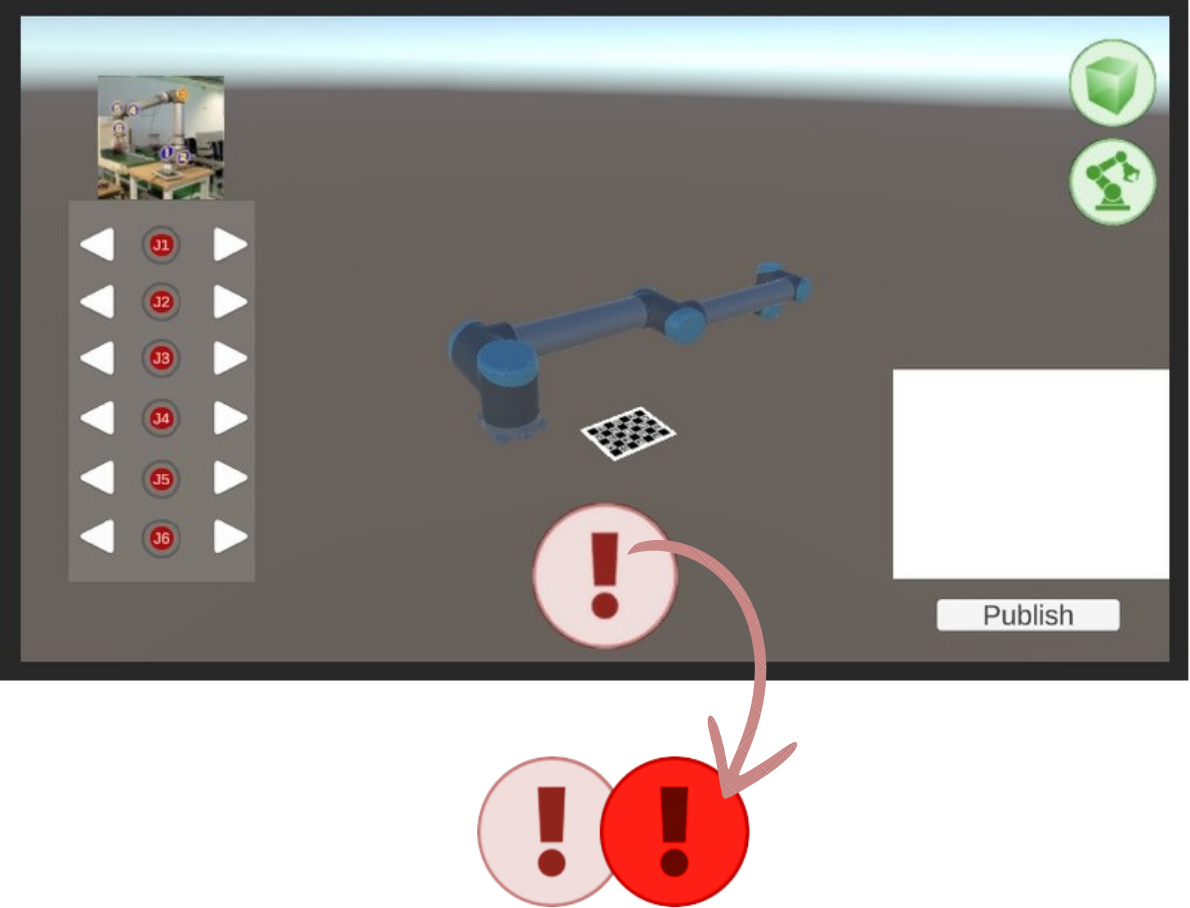
\includegraphics[width=0.7\linewidth]{figs/warning-sign.png}
        \caption{Warning blinking sign displayed in the bottom part of the \ac{UI} to alert the on-site user of proximity to the Robot}
        \label{fig:blinking-sign}
    \end{figure}

\item \textbf{Breach Protocol:} Besides the above described sensorial cues whose goal consists on improving user's awareness, another feature was implemented to ensure user's safety when interacting with the robot. If the on-site counterpart enters the Outer-Safety Zone area while the robot is in motion, the robot automatically stops. This immediate halt ensures that potential accidents or injuries are avoided by preventing any interaction with the robot when a user is within this designated dangerous area.
\end{itemize}


    
% this interface section - the feature of controlling it using the UI must be put in the UI COntrol method above
%  the remaining part should be in this part - explaining the rest of the UI features
\subsection{Interface}

% The interface, which incorporates the safety-zone features detailed earlier, is illustrated in Figure~\ref{}.
* TODO: re-do this figure with the most recent version of the UI

Besides the above described panel for controlling the digital robot's joints and the toggle button to activate/deactivate it, the interface also features another green button, designated for activating/deactivating the safety-zone functions. Upon deactivation, the button will turn gray. This design allows users to easily switch these features on or off, providing flexibility in controlling the safety mechanisms and movement operations within the \ac{MR} environment.

% \begin{figure}[h]
% \centering
% \begin{subfigure}[b]{0.31\textwidth}    
%     \centering
%     
\includegraphics[width=1\linewidth]{figs/joint-1.png}
%     \caption{Joint Control for first Joint}
%     \label{fig:joint-1}
%     \end{subfigure}
% \hfill % This command adds space between the subfigures
% \begin{subfigure}[b]{0.31\textwidth}
%     \centering
%     
\includegraphics[width=0.3\linewidth]{figs/clicked_joints.png}
%     \caption{Controller Menu Toggle}
%     \label{fig:toggle-joint}
% \end{subfigure}
% \hfill
% \begin{subfigure}[b]{0.31\textwidth}
%     \centering
%     
\includegraphics[width=0.3\linewidth]{figs/unclick_sz.png}
%     \caption{Safety-zone Toggle}
%     \label{fig:toggle-safety}
% \end{subfigure}
% \caption{Example from first joint control menu and toggle buttons for controller menu and safety-zones}
% \label{fig:joint-toggle}
% \end{figure}



% \section{Video Demo}
%     The video demonstration (\href{https://www.youtube.com/watch?v=SMQ0yXhdnUo}{https://www.youtube.com/watch?v=SMQ0yXhdnUo}) showcases 
%     the successful implementation of the previously described features. Testing of the application was conducted using a laptop paired
%      with the camera depicted in the figure \ref{fig:camera-c922}. This approach was chosen due to encountered challenges in properly
%       building the application for android \ac{HHD}.
*TODO: see this
    % this or the below commented version?
    In addition to the core controls, the \ac{UI} features a toggle button that allows the user to activate or deactivate the entire robot control panel. This is particularly useful when the user requires a larger viewport to observe the robot's movements or when switching between different control methods. When the \ac{UI} panel is hidden, the robot remains visible, but interaction via the \ac{UI} is disabled, freeing up screen space for other actions (Figure~\ref{fig:teste}). 
    % This toggle functionality also allows users to switch between different control methods while maintaining a clean and efficient workspace.

    % check which figure is this one and wheter to leave it or not?
    % \begin{figure}[h]
    % \centering
    % 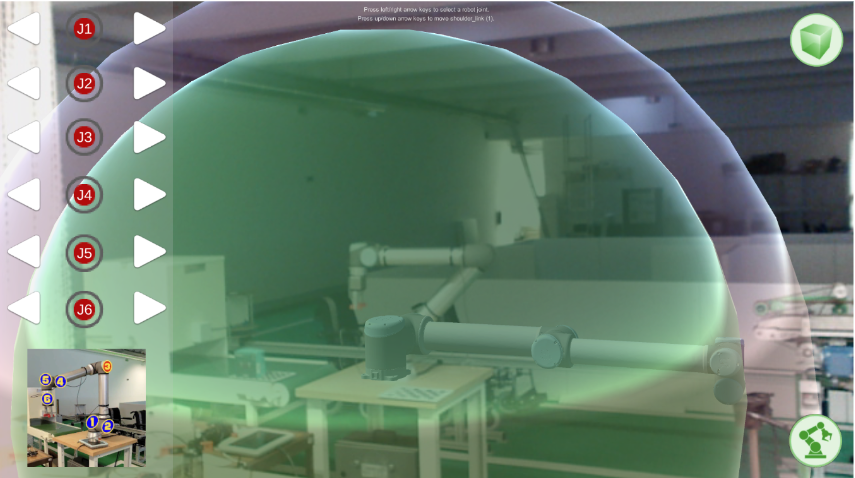
\includegraphics[width=1\linewidth]{figs/interface.png}
    % \caption{Interface featuring developed interactions}
    % \label{fig: interface}
    % \end{figure}

\begin{figure}[h]
    \centering
    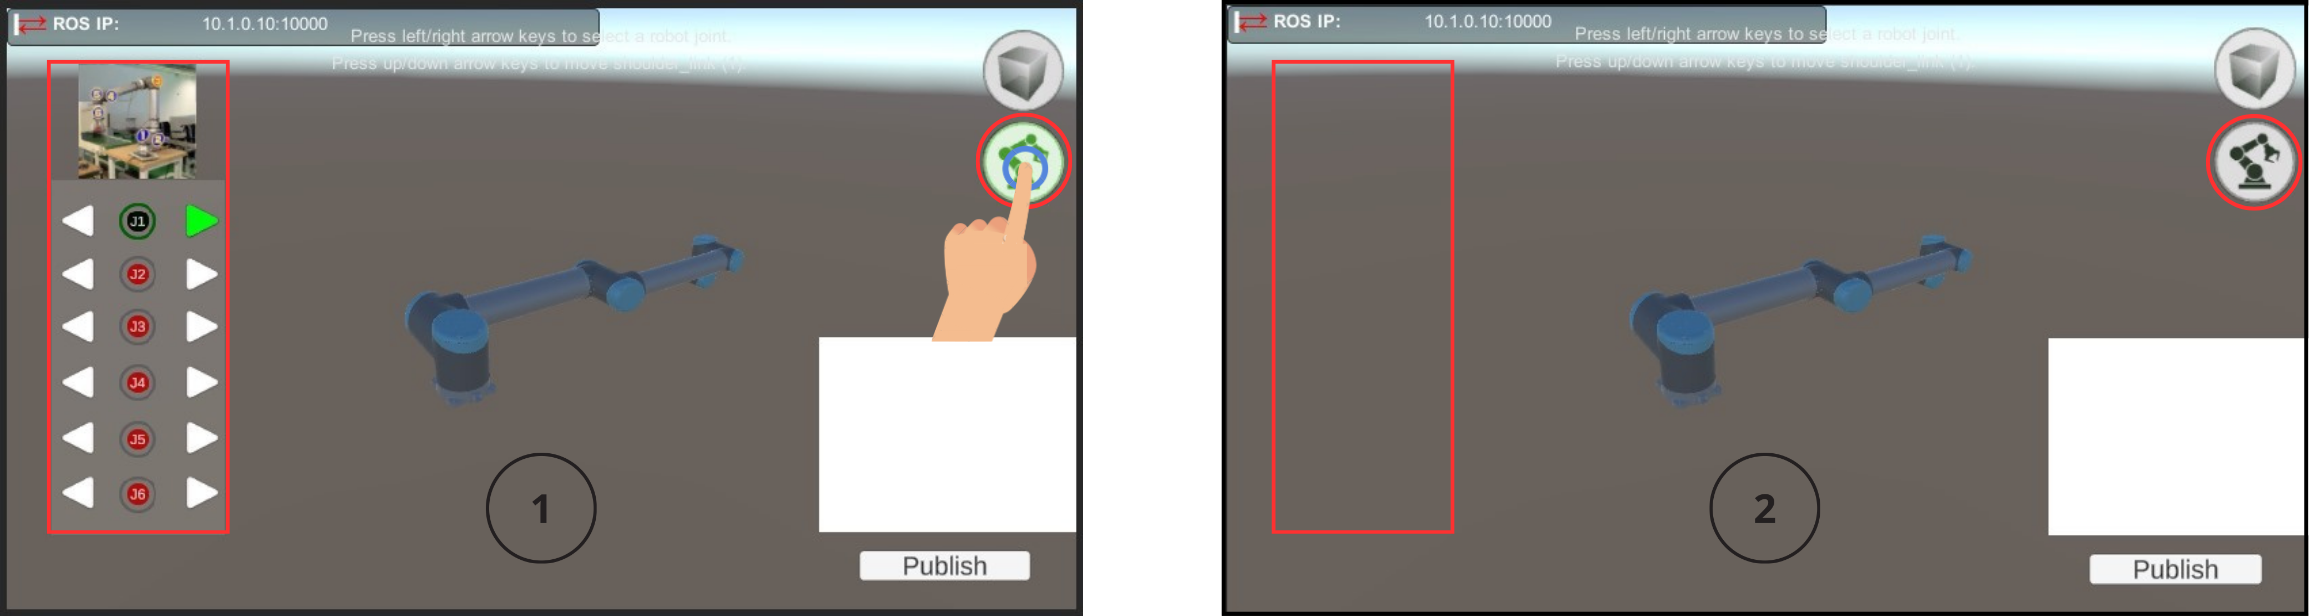
\includegraphics[width=\linewidth]{figs/mao-toca-ui-refeita-numbers.png}
    \caption{teste}
    \label{fig:teste}
\end{figure}


% continue here
\subsection{Camera Feed Transmission}

In order to enhance the remote user's understanding of the on-site environment and task performance, another camera was added, allowing for feed transmission. 

\subsubsection{Hardware and Software Setup}
An Orbbec Astra camera~\footnote{\url{https://www.orbbec.com/products/structured-light-camera/astra-series/} Acessed:2024-10-22}, displayed in the figure \ref{fig:astra-camera}, was provided by the project supervisors was used to capture the live video feed. This 3D camera was chosen for its high-quality video output and compatibility with the \ac{ROS} environment.

\begin{figure}[h]
    \centering
    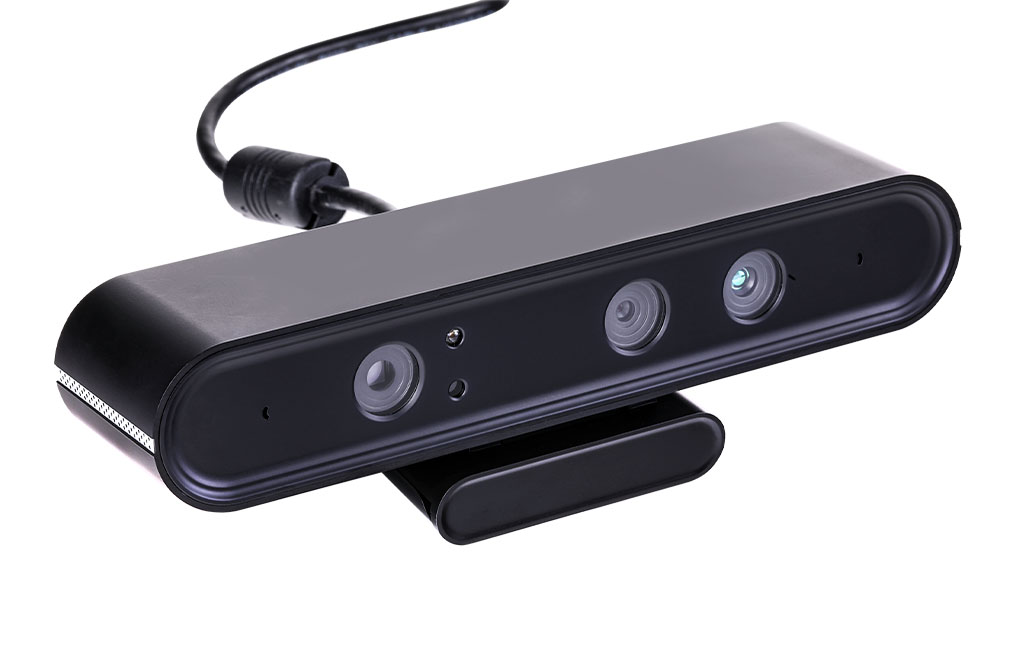
\includegraphics[width=0.5\textwidth]{figs/AstraSeries_3.jpg}
    \caption{Astra 3D Orbbec Camera used to transmit real-time video feed from robot environment to remote user}
    \label{fig:astra-camera}
\end{figure}
\FloatBarrier

To integrate the camera into the \ac{ROS} environment, an existing GitHub repository \footnote{\url{https://github.com/orbbec/ros_astra_camera} Accessed: 2024-10-04} tailored for the Astra camera integration was used. This repository contained the necessary drivers and \ac{ROS} nodes to enable the camera's functionality within the middleware framework.


\subsubsection{ROS Camera Node and Camera Transmission}

To enable the camera feed within the \ac{ROS} environment, the \texttt{astra\_camera\_node} from the \texttt{astra\_camera} package is initialized. This node captures live video data from the camera and displays it within the RViz interface to ensure the camera’s functionality and the accuracy of the captured data. This data needs to be transmitted to the Unity \ac{MR} application, allowing the remote user to observe the robot's environment in real-time, providing critical visual feedback necessary for effective remote collaboration.

However, transmitting the raw image data over the \ac{TCP} Connector/Endpoint package that enables the connection between both environments presents significant challenges due to its size and bandwidth requirements, which could affect real-time collaboration.
To overcome this, the \texttt{image\_transport} package is used. This package allows for the conversion of the raw image stream into a compressed format, reducing the data size without compromising significant image quality. In order to republish the image in a compressed format, the following \ac{ROS} command is used:

\begin{verbatim}
     rosrun image_transport republish raw 
     in:=/camera/color/image_raw out:=/camera/image_repub 
\end{verbatim}

By compressing the image data, smoother and more efficient real-time transmission to the Unity environment was achieved, ensuring minimal delay and consistent visual feedback for remote collaborators.

\subsubsection{Unity Camera Feed Integration}

After having compressed the image data, the next step was to integrate it into the Unity \ac{MR} environment. To facilitate this, a new script, \texttt{CameraFeedReceiver.cs} was developed, which handled the reception of the video feed and its subsequent rendering within the Unity application. The script was then attached to a designated \ac{UI} panel, ensuring the live camera feed could be displayed in real time for the remote users. 

*TODO: add a figure of the camera transmission in unity and rviz. should i say that it provided situational awareness of robot's surroundings, since it was not atached to the robot itself. 
The live feed provided critical situational awareness of the robot’s surroundings, aiding the remote operator in better understanding and interacting with the environment. Figure \ref{} illustrates this setup, showing the live camera feed within the Unity interface.




% To initiate the camera feed, the \texttt{astra\_camera\_node} from the \texttt{astra\_camera} package is initialized. Afterwards, an RVIZ image viewer displays the live feed, ensuring the camera is functioning correctly and capturing the desired video data.

% * TODO: add a picture of the UI showing that the camera live feed from Rviz
% * TODO: need to explain better how the image transmission is sent to the Unity, needed to compress the image data into a different format, from raw to compressed, to be able to send it over Wi-Fi - used the image\_transport package to republish the image data in a more efficient format, allowing for smoother and real-time transmission to the Unity environment.
% after launching the camera node, the image data was republished using the image\_transport package, which allowed for smoother and real-time transmission to the Unity environment.
% * TODO: reorganize this part better

% \subsection{Unity Camera Feed Integration}

% After the camera live feed was displayed in the Rviz simulation within the on-site environment, this data needs to be transmitted to the Unity \ac{MR} application, allowing the remote user to observe the robot's environment in real-time, providing critical visual feedback necessary for effective remote collaboration.


% From the Unity side, the \texttt{CameraFeedReceiver.cs} (verify the name of the script) script was developed to receive and display the live camera feed. This script was then atached to an UI interface (confirm the name of the element) that displayed the video feed in real-time. 
% add a figure of the UI interface with the view of the camera - The figure (add figure) illustrates the camera feed in the Unity application, showcasing the live video stream from the robot's environment.

% \subsection{Data Transmission to Unity} 
    
% However, the raw image data generated by the camera was too heavy to be transmitted efficiently over Wi-Fi, so this data needed to be republished using the \texttt{image\_transport} package.
% By utilizing the following \ac{ROS} command 
% \begin{verbatim}
%     rosrun image_transport republish raw 
%     in:=/camera/color/image_raw out:=/camera/image_repub
% \end{verbatim}
% the image data was republished in a more efficient format, allowing for smoother and real-time transmission to the Unity environment.

*TODO: is this useful to any integration part of this chapter???? 
The primary goal of this project consists on enhancing remote collaboration between human operators by utilizing a robotic arm (UR10e) and \ac{MR}. In order to achieve this, a framework allowing for an interactive, fully functional \ac{MR} application that facilitates bidirectional communication between the robot and its \ac{DT} was developed. It features a friendly \ac{UI} that enables the visualization and control of the robotic arm, where the \ac{DT} was designed to respond in real-time to the robot's physical movements, and vice versa. The achieved bidirectional communication ensures that the \ac{MR} system operates not as a mere digital shadow of the robot but as a true \ac{DT}, capable of reflecting and influencing the physical entity.

One of the key features developed was a seamless control method integrated within the \ac{MR} environment, allowing the user to manipulate the robot via the \ac{UI}. This interface includes joint's selection buttons, directional controls, and toggle switches for precise manipulation of each robotic joint.  This setup enables users to control the robot's movements through the \ac{MR} interface and send this position update to the \ac{ROS} middleware, with real-time synchronization ensuring the robot accurately mirrors the \ac{DT}'s state.

The development of two safety zones within the \ac{UI} was a critical enhancement aimed at ensuring user safety and improving operational awareness when interacting with the robot. These zones function by providing real-time alerts to the user. When the user enters the "Outer Safety Zone", which has a larger radius, not only a visual alert starts blinking, but also the color of the "Inner Safety Zone" changes, signaling that the user is approaching the robot's workspace. These visual cue escalate the user's awareness of proximity to the robot. If he gets even closer to the robot and breaches the "Inner Safety Zone", an auditory alarm is triggered, continuously alerting the user to their presence within a hazardous area. This layered approach—combining visual color changes and auditory alarms—ensures that users are fully aware of any potential danger during robot operation, thereby preventing accidents. Moreover, the combination of these sensorial cues also contributes to a more immersive interaction experience, increasing awareness without overwhelming the user.
However, the accuracy of these safety zones is heavily dependent on the alignment between the camera and the \ac{AR} marker. Misalignment between the them can lead to inaccuracies in distance measurements, affecting the reliability of the safety zones. Maintaining precise marker tracking is therefore essential for ensuring both the accuracy of safety zone alerts and the overall safety of the system during operation.

Another significant feature was the implementation of a live camera feed, allowing the remote participant to view the robot’s workspace in real-time. This feed is crucial for remote collaboration, enabling users from different locations to have a synchronized understanding of the robot’s surroundings. The camera feed is transmitted from the \ac{ROS} middleware to the Unity \ac{MR} environment via \ac{TCP}/\ac{IP} after image compression. Compression was necessary due to the substantial bandwidth required for raw video data transmission. This feature offers an important perspective for remote users, aiding in monitoring and providing assistance when necessary.

Both the joint control interface and the safety-zone mechanisms were designed to be toggled on/off, thereby ensuring that the user has the option to clear the \ac{UI} for an unobstructed view of the environment.

